%%%%%%%%%%%%%%%%%%%%%%%%%%%%%%%%%%%%%%%%%%%%%%%%%%%%%%%%%%%%%%%%%%%%%%%%%%%%%%%%%%%%%%%%%%%%%%%%%%%%%%%%%%%%%%%%%%%%%%%%%%%%%%%%%%%%%%%%%%%%%%%%%%%%%%%%%%%%%%%%%%%
% Written By Michael Brodskiy
% Class: General Relativity and Cosmology
% Professor: J. Blazek
%%%%%%%%%%%%%%%%%%%%%%%%%%%%%%%%%%%%%%%%%%%%%%%%%%%%%%%%%%%%%%%%%%%%%%%%%%%%%%%%%%%%%%%%%%%%%%%%%%%%%%%%%%%%%%%%%%%%%%%%%%%%%%%%%%%%%%%%%%%%%%%%%%%%%%%%%%%%%%%%%%%

\include{Includes.tex}

\title{Lecture 1}
\date{\today}
\author{Michael Brodskiy\\ \small Professor: J. Blazek}

\begin{document}

\maketitle

\begin{itemize}

  \item The Equivalence Principle (for all freely-falling reference frames)

    \begin{itemize}

      \item General Relativity $>$ Special Relativity

    \end{itemize}

  \item Geodesic — The shortest realizable line between two points

  \item Beyond Newton — Gravity as Geometry

    \begin{itemize}

      \item Einstein's Equation

        $$\nabla^2\Phi=4\pi G\rho\to G_{\mu v}=R_{\mu v}-\frac{1}{2}Rg_{\mu v}=8\pi GT_{\mu v}$$

    \end{itemize}

  \item Accelerating Universe (Cosmological Constant? Dark Energy?)

    $$R_{\mu v}-\frac{1}{2} Rg_{\mu v}+\Lambda g_{\mu v}=8\pi GT_{\mu v}$$

  \item Dark Matter

  \item Cosmic Microwave Background (CMB)

  \item Galaxy Clustering

  \item Gravitational Lensing

  \item Gravitational Waves

  \item Special Relativity Review

    \begin{itemize}

      \item Main Tenets (Einstein's Postulates)

        \begin{itemize}

          \item Laws of Physics are the same in all inertial reference frames
    
          \item The speed of light is invariable (always $c$)

            \begin{itemize}

              \item $c$ is the maximum observable speed

            \end{itemize}

        \end{itemize}

      \item Phenomena Explained by Special Relativity

        \begin{itemize}

          \item Loss of Simultaneity

          \item Length contraction/dilation

          \item Time contraction/dilation (Twin Paradox)

          \item Magnetic $\leftrightarrow$ Electric fields

          \item Velocity addition ($v_{t}\neq v_1+v_2$)

        \end{itemize}

      \item Paradoxes

        \begin{itemize}

          \item Twin Paradox

            \begin{itemize}

              \item Two twins, one who stays on Earth, and one who flies to space and returns. The twin who stayed on Earth ages faster relative to the twin in space. To both, it appears that the other ages slower

              \item Acceleration means the twin who ``goes'' is not always in an inertial frame

            \end{itemize}

          \item Pole-vaulter Paradox

            \begin{itemize}

              \item A pole-vaulter with a pole longer than a barn can make it through the barn, even when the doors appear to open and close at the same time for a stationary observer. This is because of the loss of simultaneity; that is, for the vaulter the doors open and close at different times

            \end{itemize}

        \end{itemize}

    \end{itemize}

  \item Light clock derivation of time dilation

    \begin{itemize}

      \item To keep time, light is sent from one mirror to another. A counter counts each time light hits the bottom mirror. The two mirrors are separated by length $L$

      \item Time is kept with ``cycles'' of how long it takes light to travel from one mirror to the other

      \item When stationary, a cycle is:

        $$T=\frac{2L}{c}$$

      \item If a stationary observer sees the light clock move, with some velocity $v$, the light appears to form a triangle pattern, shown in Figure \ref{fig:1} below:

        \begin{figure}[h]
          \centering
          \tikzset{every picture/.style={line width=0.75pt}} %set default line width to 0.75pt        

\begin{tikzpicture}[x=0.75pt,y=0.75pt,yscale=-1,xscale=1]
%uncomment if require: \path (0,300); %set diagram left start at 0, and has height of 300

%Straight Lines [id:da6024213712431123] 
\draw    (223.29,79) -- (81.87,79) ;
%Straight Lines [id:da8694164398690145] 
\draw    (364.71,2) -- (223.29,2) ;
%Straight Lines [id:da4213047654494104] 
\draw    (506.13,79) -- (364.71,79) ;
%Straight Lines [id:da20517294265853447] 
\draw [color={rgb, 255:red, 74; green, 144; blue, 226 }  ,draw opacity=1 ][fill={rgb, 255:red, 248; green, 231; blue, 28 }  ,fill opacity=1 ]   (152.58,79) -- (292.24,2.96) ;
\draw [shift={(294,2)}, rotate = 151.43] [color={rgb, 255:red, 74; green, 144; blue, 226 }  ,draw opacity=1 ][line width=0.75]    (10.93,-3.29) .. controls (6.95,-1.4) and (3.31,-0.3) .. (0,0) .. controls (3.31,0.3) and (6.95,1.4) .. (10.93,3.29)   ;
%Straight Lines [id:da7921750006687314] 
\draw [color={rgb, 255:red, 74; green, 144; blue, 226 }  ,draw opacity=1 ]   (294,2) -- (433.66,78.04) ;
\draw [shift={(435.42,79)}, rotate = 208.57] [color={rgb, 255:red, 74; green, 144; blue, 226 }  ,draw opacity=1 ][line width=0.75]    (10.93,-3.29) .. controls (6.95,-1.4) and (3.31,-0.3) .. (0,0) .. controls (3.31,0.3) and (6.95,1.4) .. (10.93,3.29)   ;
%Straight Lines [id:da22199529653547656] 
\draw [color={rgb, 255:red, 208; green, 2; blue, 27 }  ,draw opacity=1 ]   (67.03,4) -- (67.97,77) ;
\draw [shift={(68,79)}, rotate = 269.26] [color={rgb, 255:red, 208; green, 2; blue, 27 }  ,draw opacity=1 ][line width=0.75]    (10.93,-3.29) .. controls (6.95,-1.4) and (3.31,-0.3) .. (0,0) .. controls (3.31,0.3) and (6.95,1.4) .. (10.93,3.29)   ;
\draw [shift={(67,2)}, rotate = 89.26] [color={rgb, 255:red, 208; green, 2; blue, 27 }  ,draw opacity=1 ][line width=0.75]    (10.93,-3.29) .. controls (6.95,-1.4) and (3.31,-0.3) .. (0,0) .. controls (3.31,0.3) and (6.95,1.4) .. (10.93,3.29)   ;

% Text Node
\draw (65.5,40.5) node [anchor=east] [inner sep=0.75pt]    {$L$};


\end{tikzpicture}

          \caption{A Moving Light Clock from Stationary Reference Frame}
          \label{fig:1}
        \end{figure}

        \begin{itemize}

          \item From the set up, it can be determined that the observed change in time for one individual can be expressed as a function of the change in time observed by the moving individual, times $\gamma$, where:

            $$\gamma=\frac{1}{\sqrt{1-\left( \frac{v}{c} \right)^2}}$$
            $$\Delta t'=\gamma\Delta t$$

          \item Thus, we see that at $v=0:\gamma=1$ and at $v\to c:\gamma\to\infty$

        \end{itemize}

    \end{itemize}

  \item Lorentz Transformations and Rotations

    \begin{figure}[H]
      \centering
      \tikzset{every picture/.style={line width=0.75pt}} %set default line width to 0.75pt        

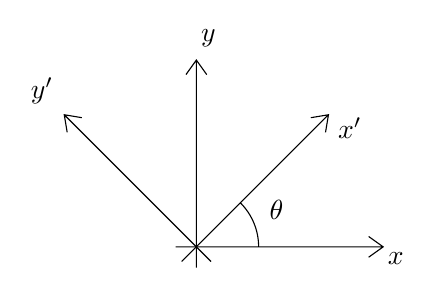
\begin{tikzpicture}[x=0.75pt,y=0.75pt,yscale=-1,xscale=1]
%uncomment if require: \path (0,300); %set diagram left start at 0, and has height of 300

%Shape: Axis 2D [id:dp6052588153202806] 
\draw  (214,173) -- (314,173)(224,83) -- (224,183) (307,168) -- (314,173) -- (307,178) (219,90) -- (224,83) -- (229,90)  ;
%Shape: Axis 2D [id:dp2386863255816345] 
\draw  (216.93,180.07) -- (287.64,109.36)(160.36,109.36) -- (231.07,180.07) (279.15,110.77) -- (287.64,109.36) -- (286.23,117.85) (161.77,117.85) -- (160.36,109.36) -- (168.85,110.77)  ;
%Shape: Arc [id:dp02254630738242136] 
\draw  [draw opacity=0] (245.21,151.79) .. controls (245.21,151.79) and (245.21,151.79) .. (245.21,151.79) .. controls (245.21,151.79) and (245.21,151.79) .. (245.21,151.79) .. controls (251.07,157.64) and (254,165.32) .. (254,173) -- (224,173) -- cycle ; \draw   (245.21,151.79) .. controls (245.21,151.79) and (245.21,151.79) .. (245.21,151.79) .. controls (245.21,151.79) and (245.21,151.79) .. (245.21,151.79) .. controls (251.07,157.64) and (254,165.32) .. (254,173) ;  

% Text Node
\draw (225,78) node [anchor=south west] [inner sep=0.75pt]    {$y$};
% Text Node
\draw (315,174.4) node [anchor=north west][inner sep=0.75pt]    {$x$};
% Text Node
\draw (291,109.4) node [anchor=north west][inner sep=0.75pt]    {$x'$};
% Text Node
\draw (143,90.4) node [anchor=north west][inner sep=0.75pt]    {$y'$};
% Text Node
\draw (258,149.4) node [anchor=north west][inner sep=0.75pt]    {$\theta $};


\end{tikzpicture}

      \caption{Rotation of Coordinate System}
      \label{fig:2}
    \end{figure}

    \begin{itemize}

      \item Following rotation, we get:

        $$x'=x\cos(\theta)-y\sin(\theta)$$
        $$y'=x\sin(\theta)+y\cos(\theta)$$

      \item For boosting in a single direction (``rotation'' between space and time):

        $$x'=(x-vt)\gamma$$
        $$y'=y$$
        $$z'=z$$
        $$t'=(t-vx)\gamma$$

      \item Space and time are no longer separate $\Rightarrow$ single spacetime

      \item A translation would involve movement of the origin

    \end{itemize}

  \item Spacetime Diagram

    \begin{figure}[H]
      \centering
      \tikzset{every picture/.style={line width=0.75pt}} %set default line width to 0.75pt        

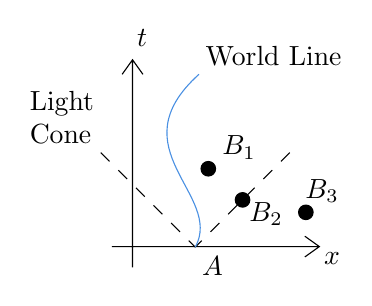
\begin{tikzpicture}[x=0.75pt,y=0.75pt,yscale=-1,xscale=1]
%uncomment if require: \path (0,300); %set diagram left start at 0, and has height of 300

%Shape: Axis 2D [id:dp6052588153202806] 
\draw  (214,173) -- (314,173)(224,83) -- (224,183) (307,168) -- (314,173) -- (307,178) (219,90) -- (224,83) -- (229,90)  ;
%Straight Lines [id:da10036025459043973] 
\draw  [dash pattern={on 4.5pt off 4.5pt}]  (299.78,127.72) -- (254.22,173.28) ;
%Straight Lines [id:da6125249800197986] 
\draw  [dash pattern={on 4.5pt off 4.5pt}]  (208.67,127.72) -- (254.22,173.28) ;
%Shape: Circle [id:dp934318391813717] 
\draw  [fill={rgb, 255:red, 0; green, 0; blue, 0 }  ,fill opacity=1 ] (257,135.5) .. controls (257,133.57) and (258.57,132) .. (260.5,132) .. controls (262.43,132) and (264,133.57) .. (264,135.5) .. controls (264,137.43) and (262.43,139) .. (260.5,139) .. controls (258.57,139) and (257,137.43) .. (257,135.5) -- cycle ;
%Shape: Circle [id:dp8271827138927054] 
\draw  [fill={rgb, 255:red, 0; green, 0; blue, 0 }  ,fill opacity=1 ] (273.5,150.5) .. controls (273.5,148.57) and (275.07,147) .. (277,147) .. controls (278.93,147) and (280.5,148.57) .. (280.5,150.5) .. controls (280.5,152.43) and (278.93,154) .. (277,154) .. controls (275.07,154) and (273.5,152.43) .. (273.5,150.5) -- cycle ;
%Shape: Circle [id:dp6545413454296474] 
\draw  [fill={rgb, 255:red, 0; green, 0; blue, 0 }  ,fill opacity=1 ] (304,156.5) .. controls (304,154.57) and (305.57,153) .. (307.5,153) .. controls (309.43,153) and (311,154.57) .. (311,156.5) .. controls (311,158.43) and (309.43,160) .. (307.5,160) .. controls (305.57,160) and (304,158.43) .. (304,156.5) -- cycle ;
%Curve Lines [id:da7989853479672057] 
\draw [color={rgb, 255:red, 74; green, 144; blue, 226 }  ,draw opacity=1 ]   (254.22,173.28) .. controls (268,148) and (216,126) .. (256,90) ;

% Text Node
\draw (225,78) node [anchor=south west] [inner sep=0.75pt]    {$t$};
% Text Node
\draw (315,174.4) node [anchor=north west][inner sep=0.75pt]    {$x$};
% Text Node
\draw (206.67,124.72) node [anchor=south east] [inner sep=0.75pt]   [align=left] {Light \\Cone};
% Text Node
\draw (256.22,176.68) node [anchor=north west][inner sep=0.75pt]    {$A$};
% Text Node
\draw (266,132.1) node [anchor=south west] [inner sep=0.75pt]    {$B_{1}$};
% Text Node
\draw (279,150.4) node [anchor=north west][inner sep=0.75pt]    {$B_{2}$};
% Text Node
\draw (306,153.1) node [anchor=south west] [inner sep=0.75pt]    {$B_{3}$};
% Text Node
\draw (258,87) node [anchor=south west] [inner sep=0.75pt]   [align=left] {World Line};


\end{tikzpicture}

      \caption{Example Spacetime Diagram}
      \label{fig:3}
    \end{figure}

    \begin{itemize}

      \item Points represent events

      \item Light always travels at $45^{\circ}$

      \item Cone of causality: outside cone is causally separate (events inside cone can not affect events outside of it)

      \item Inside a light cone, it is possible to perform a boost such that events happen in the same place

      \item Lorentz transformation ``squeezes'' axes

        \begin{figure}[H]
          \centering
          \tikzset{every picture/.style={line width=0.75pt}} %set default line width to 0.75pt        

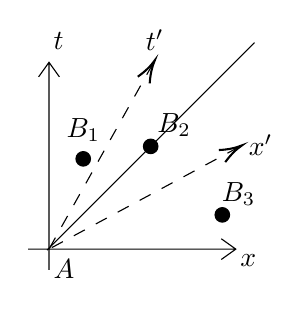
\begin{tikzpicture}[x=0.75pt,y=0.75pt,yscale=-1,xscale=1]
%uncomment if require: \path (0,300); %set diagram left start at 0, and has height of 300

%Shape: Axis 2D [id:dp6052588153202806] 
\draw  (214,173) -- (314,173)(224,83) -- (224,183) (307,168) -- (314,173) -- (307,178) (219,90) -- (224,83) -- (229,90)  ;
%Straight Lines [id:da10036025459043973] 
\draw  [dash pattern={on 4.5pt off 4.5pt}]  (315.24,123.95) -- (224,173) ;
\draw [shift={(317,123)}, rotate = 151.74] [color={rgb, 255:red, 0; green, 0; blue, 0 }  ][line width=0.75]    (10.93,-3.29) .. controls (6.95,-1.4) and (3.31,-0.3) .. (0,0) .. controls (3.31,0.3) and (6.95,1.4) .. (10.93,3.29)   ;
%Straight Lines [id:da6125249800197986] 
\draw  [dash pattern={on 4.5pt off 4.5pt}]  (274.02,83.74) -- (224,173) ;
\draw [shift={(275,82)}, rotate = 119.27] [color={rgb, 255:red, 0; green, 0; blue, 0 }  ][line width=0.75]    (10.93,-3.29) .. controls (6.95,-1.4) and (3.31,-0.3) .. (0,0) .. controls (3.31,0.3) and (6.95,1.4) .. (10.93,3.29)   ;
%Shape: Circle [id:dp934318391813717] 
\draw  [fill={rgb, 255:red, 0; green, 0; blue, 0 }  ,fill opacity=1 ] (237,129.5) .. controls (237,127.57) and (238.57,126) .. (240.5,126) .. controls (242.43,126) and (244,127.57) .. (244,129.5) .. controls (244,131.43) and (242.43,133) .. (240.5,133) .. controls (238.57,133) and (237,131.43) .. (237,129.5) -- cycle ;
%Shape: Circle [id:dp8271827138927054] 
\draw  [fill={rgb, 255:red, 0; green, 0; blue, 0 }  ,fill opacity=1 ] (269.5,123.5) .. controls (269.5,121.57) and (271.07,120) .. (273,120) .. controls (274.93,120) and (276.5,121.57) .. (276.5,123.5) .. controls (276.5,125.43) and (274.93,127) .. (273,127) .. controls (271.07,127) and (269.5,125.43) .. (269.5,123.5) -- cycle ;
%Shape: Circle [id:dp6545413454296474] 
\draw  [fill={rgb, 255:red, 0; green, 0; blue, 0 }  ,fill opacity=1 ] (304,156.5) .. controls (304,154.57) and (305.57,153) .. (307.5,153) .. controls (309.43,153) and (311,154.57) .. (311,156.5) .. controls (311,158.43) and (309.43,160) .. (307.5,160) .. controls (305.57,160) and (304,158.43) .. (304,156.5) -- cycle ;
%Straight Lines [id:da34724223215423533] 
\draw    (323,73.5) -- (223,173.5) ;

% Text Node
\draw (225,78) node [anchor=south west] [inner sep=0.75pt]    {$t$};
% Text Node
\draw (315,174.4) node [anchor=north west][inner sep=0.75pt]    {$x$};
% Text Node
\draw (225,176.9) node [anchor=north west][inner sep=0.75pt]    {$A$};
% Text Node
\draw (240.5,122.6) node [anchor=south] [inner sep=0.75pt]    {$B_{1}$};
% Text Node
\draw (275,120.1) node [anchor=south west] [inner sep=0.75pt]    {$B_{2}$};
% Text Node
\draw (306,153.1) node [anchor=south west] [inner sep=0.75pt]    {$B_{3}$};
% Text Node
\draw (275,78.6) node [anchor=south] [inner sep=0.75pt]    {$t'$};
% Text Node
\draw (319,123) node [anchor=west] [inner sep=0.75pt]    {$x'$};


\end{tikzpicture}

          \caption{Lorentz Transformation from $O$ to $O'$}
          \label{fig:4}
        \end{figure}

      \item $A$ to $B_1$: $\Delta t$ and $\Delta t'$ are positive

      \item $A$ to $B_2$:  $\Delta x=\Delta t$, $\Delta x'=\Delta t'$

      \item $A$ to $B_3$: $\Delta x$, $\Delta x'$ are positive

      \item Distances are invariant under translations and rotations (in standard Euclidean space)

      \item Distances in spacetime: spacetime interval
        
        \begin{itemize}

          \item For flat space (Minkowski space)

            $$\Delta s^2=-\Delta t^2+\Delta x^2 + \Delta y^2+\Delta z^2$$

            \begin{itemize}

              \item Has a $-+++$ signature, versus a $+---$ signature

              \item If $\Delta s^2<0$: time-like separation

              \item If $\Delta s^2=0$: light-like (null) separation

              \item If $\Delta s^2>0$: space-like separation

              \item With proper time $\tau$:

                $$\Delta \tau^2=-\Delta s^2$$

            \end{itemize}

        \end{itemize}

    \end{itemize}

  \item Changing between inertial reference frams is a Lorentz transformation

    \begin{itemize}

      \item $\Delta s$ is invariant under Lorentz transformations

      \item General Relativity involves generalizing this to curved space $\Rightarrow$ differential geometry

    \end{itemize}

\end{itemize}

\end{document}

